%20 min preso!
\documentclass[xcolor=table]{beamer}
\usepackage{beamerthemesplit}
\usepackage{wrapfig}
\usetheme{SPbGU}
\usepackage{pdfpages}
\usepackage{amsmath}
\usepackage{cmap}
\usepackage[T2A]{fontenc}
\usepackage[utf8]{inputenc}
\usepackage[english]{babel}
\usepackage{indentfirst}
\usepackage{amsmath}
\usepackage{tikz}
\usepackage{multirow}
\usepackage[noend]{algpseudocode}
\usepackage{algorithm}
\usepackage{algorithmicx}
\usepackage{fancyvrb}
\usetikzlibrary{calc}
\usetikzlibrary{shapes,arrows}
\usetikzlibrary{arrows,automata}
\usetikzlibrary{positioning}

\usepackage{tabularx}
\newcolumntype{Y}{>{\raggedleft\arraybackslash}X}


\newtheorem{mytheorem}{Theorem}
\renewcommand{\thealgorithm}{}

\newcommand{\tikzmark}[1]{\tikz[overlay,remember picture] \node (#1) {};}
\def\Put(#1,#2)#3{\leavevmode\makebox(0,0){\put(#1,#2){#3}}}

\tikzset{
    state/.style={
           rectangle,
           rounded corners,
           draw=black, very thick,
           minimum height=2em,
           inner sep=2pt,
           text centered,
           },
}

\beamertemplatenavigationsymbolsempty

\title[DNN + Formal Grammars]{The Composition of Dense Neural Networks and Formal~Grammars for Secondary Structure Analysis}
%\subtitle[YaccConstructor]{Parsing techniques for graph analysis}
% То, что в квадратных скобках, отображается в левом нижнем углу.
\institute[JetBrains Research]{
JetBrains Research, Programming Languages and Tools Lab  \\
Saint Petersburg University
}

% То, что в квадратных скобках, отображается в левом нижнем углу.
\author[Semyon Grigorev]{Polina Lunina, \textbf{Semyon Grigorev}}

\date{Febrary 24, 2019}

\begin{document}
{
\begin{frame}[fragile]
  \begin{table}
  \centering
  \begin{tabularx}{\linewidth}{YcX}
    
\includegraphics[height=1.5cm]{pictures/jetbrainsResearch.pdf} \hfill
    & \begin{minipage}[t]{0.3\textwidth}\center \vspace{-1cm}  BIOINFORMATICS 2019
      \end{minipage}
    & \hfill 
\includegraphics[height=1.5cm]{pictures/SPbGU_Logo.png}
  \end{tabularx}
  \end{table}
  \titlepage
\end{frame}
}

\begin{frame} \frametitle{Sequences Analysis: classification, search\dots}

\begin{minipage}[t]{0.49\textwidth}
\textbf{Problem: high variability of data}
\begin{itemize}
   \item Mutations
   \item Different kinds of noise
   \item \dots
\end{itemize}
\pause
\textbf{We need probabilistic approaches}
\end{minipage}
\pause
~
\begin{minipage}[t]{0.47\textwidth}
\textbf{Level of abstraction}
\begin{itemize}
   \item Primary structure
   \item Secondary structure
   \item Tertiary structure
\end{itemize}
\pause
\textbf{We should handle secondary structure}
\end{minipage}


{
\begin{center}
\pause
\vspace{1cm}
\textbf{Probabilistic approach which handles secondary structure}
\end{center}
}
\end{frame}


%\begin{frame} \frametitle{Probabilistic approaches}

%\begin{itemize}
  %\item Hidden Markov's Models (HMM's)
  %\item Probabilistic grammars (Secondary structure)
  %item Covariation Models (CM's) (Secondary structure)
  %item Artificial neural networks (Basicly no)
%\end{itemize}
%
%\end{frame}


\begin{frame} \frametitle{Proposed Solution: Parsing + Artificial Neural Network}

\begin{itemize}
  \item Use parsing to extract features, not to model secondary structure
  \begin{itemize}
    \item As compared to the classical way of probabilistic CF grammars utilization
  \end{itemize}
  \pause
  \item Formal grammars as secondary structure description
  \item Parsing as features extraction
  \item Artificial neural network as probabilistic model for features processing
\end{itemize}

\end{frame}


\begin{frame} \frametitle{Solution Structure}
\tiny %\hspace{-2cm}
  \begin{tikzpicture}[->,>=stealth']


  \node[state,
        align=left,
        text width = 3.5cm] (grm)
   {
    \textbf{Grammar}\\
  Fixed formal grammar (not necessarily context-free) describes features of secondary structure and can be tuned to increase the quality of result.

   };


  \node[state,
        below of=grm,
        node distance=1.5cm,
        align = left,
        text width = 3.5cm] (sqs)
   {
   \textbf{Sequences}\\
  Each sequence is treated as a text in $\{A, C, G, T\}$ alphabet.
   };


  \node[state,
        right of=grm,
        node distance=4cm,
        align = left,
        text width = 3.5cm](parser)
  {
  \textbf{Parser}\\
  Parser extracts features of the given sequence secondary structure.
  Implementation of parsing algorithm is based on matrix multiplications (Valiant, Okhotin) and utilizes GPGPU.
  };

  \node[state,
        right of=parser,
        node distance=4cm,
        align = left,
        text width = 3.5cm] (mtrx)
  {
    \textbf{Matrices}\\
    %\vspace{0.05cm}
    \[ \left( \begin{array}{cccc}
    0 & \textbf{1} & 0 & \textbf{1}\\
    0 & 0 & \textbf{1} & 0\\
    0 & 0 & 0 & \textbf{1}\\
    0 & 0 & 0 & 0
    \end{array} \right)\]
    \vspace{-0.1cm}

  Parsing result is (0-1) matrix~$M$ which represents secondary structure features for sequence $\omega$: $ M[i,j] = 1 \iff \text{\ttfamily{s1}} \xrightarrow{*}{} \omega[i,j]$, and $0$ otherwise.
  };

  \node[state,
        below of=sqs,
        node distance=1cm,
        align = left,
        text width = 3.5cm](result)
  {
  \textbf{Result of classification}

  };


  \node[state,
        below of=parser,
        node distance=4.2cm,
        align = left,
        text width = 3.5cm](DNN)
  {
  \textbf{Neural Network}\\

  Dense neural network with more than 10 dense layers.
  Agressive dropout and batch normalization for learning process stabilization.\\
  Typical building block:
  \\
  \vspace{-0.3cm}
  \begin{center}
  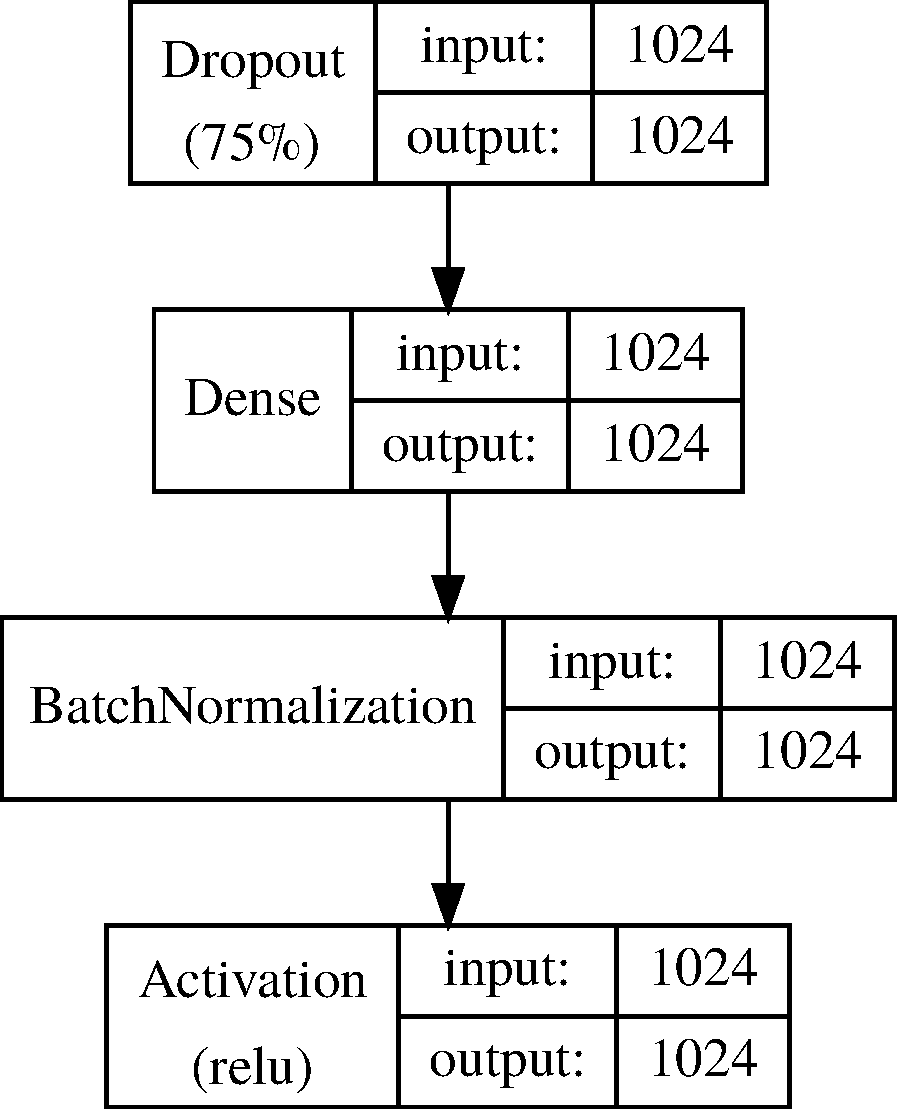
\includegraphics[width=2.5cm]{pictures/bb.pdf}
  \end{center}

  };


  \node[state,
        right of=DNN,
        node distance=4cm,
        align = left,
        text width = 3.5cm](vector)
  {
  \textbf{Vectors}\\
  \vspace{-0.1cm}

\[ \left( \begin{array}{cccc}
0 & 1 & 0 & 1\\
0 & 0 & 1 & 0\\
0 & 0 & 0 & 1\\
0 & 0 & 0 & 0
\end{array} \right) \]
\vspace{-0.35cm}
$$\Downarrow$$
\vspace{-0.35cm}
$$\texttt{[0,1,0,1,0,1,0,0,1,0]}$$
\vspace{-0.35cm}
$$\Downarrow$$
\vspace{-0.35cm}
$$\texttt{[84,128]}$$
%\vspace{-0.1cm}
  Line-by-line compressed matrix representation: sequence of 8 cells (bits) is compressed into a byte. Bottom left triangle of the matrix is always empty, so can be ignored.
  };


  \path (grm) edge  (parser)
   (sqs) edge [bend right] (parser)
  % (sqs) edge (parser)
   (parser) edge (mtrx)
   (mtrx) edge (vector)
   (vector) edge (DNN)
   (DNN) edge (result)
   ;

  \end{tikzpicture}

  \tikzmark{zzz}{
  }
  %}
  \pause
  \onslide<2>{\tikz[overlay,remember picture]{\draw[draw=red,thick,double,fill opacity=0.2] ($ (zzz) + (-0.1,7.9)$) rectangle ($ (zzz) + (3.8,4.8)$);}}

  \onslide<3>{\tikz[overlay,remember picture]{\draw[draw=red,thick,double,fill opacity=0.2] ($ (zzz) + (3.8,7.9)$) rectangle ($ (zzz) + (7.8,5.9)$);}}

  \onslide<4>{\tikz[overlay,remember picture]{\draw[draw=red,thick,double,fill opacity=0.2] ($ (zzz) + (7.8,8.5)$) rectangle ($ (zzz) + (11.8,5.25)$);}}

  \onslide<5>{\tikz[overlay,remember picture]{\draw[draw=red,thick,double,fill opacity=0.2] ($ (zzz) + (7.8,5.1)$) rectangle ($ (zzz) + (11.8,0.35)$);}}

  \onslide<6>{\tikz[overlay,remember picture]{\draw[draw=red,thick,double,fill opacity=0.2] ($ (zzz) + (3.9,5.2)$) rectangle ($ (zzz) + (7.8,0.2)$);}}

  \onslide<7>{\tikz[overlay,remember picture]{\draw[draw=red,thick,double,fill opacity=0.2] ($ (zzz) + (-0.1,4.8)$) rectangle ($ (zzz) + (3.8,4.0)$);}}


\end{frame}

\begin{frame}[fragile] \frametitle{Grammar}
%\onslide<1-4>{

\begin{verbatim}
s1: stem<s0>
any_str: any_smb*[2..10]
any_smb: A | T | C | G
stem1<s>:               \\ stem of height exactly 1
      A s T | T s A | C s G | G s C
stem3<s>:               \\ stem of height exactly 3
      stem1< stem1< stem1<s> > >
stem<s>:                \\ stem of height 3 or more
      A stem<s> T
    | T stem<s> A
    | C stem<s> G
    | G stem<s> C
    | stem3<s>
s0: any_str | any_str stem<s0> s0
\end{verbatim}
\tikzmark{yyy}{
}
%}
\pause
\onslide<2>{\tikz[overlay,remember picture]{\draw[draw=red,thick,double,fill opacity=0.2] ($ (yyy) + (-0.2,7.5)$) rectangle ($ (yyy) + (12,7)$);}}
\onslide<3>{\tikz[overlay,remember picture]{\draw[draw=red,thick,double,fill opacity=0.2] ($ (yyy) + (-0.2,7)$) rectangle ($ (yyy) + (12,6)$);}}
\onslide<4>{\tikz[overlay,remember picture]{\draw[draw=red,thick,double,fill opacity=0.2] ($ (yyy) + (-0.2,6)$) rectangle ($ (yyy) + (12,5.1)$);}}
\onslide<5>{\tikz[overlay,remember picture]{\draw[draw=red,thick,double,fill opacity=0.2] ($ (yyy) + (-0.2,5.1)$) rectangle ($ (yyy) + (12,4.1)$);}}
\onslide<6>{\tikz[overlay,remember picture]{\draw[draw=red,thick,double,fill opacity=0.2] ($ (yyy) + (-0.2,4.1)$) rectangle ($ (yyy) + (12,1.2)$);}}
\onslide<7>{\tikz[overlay,remember picture]{\draw[draw=red,thick,double,fill opacity=0.2] ($ (yyy) + (-0.2,1.2)$) rectangle ($ (yyy) + (12,0.7)$);}}
\end{frame}

\begin{frame}[fragile] \frametitle{Example 1: Stem}
\centering
 \texttt{CCCC{\color{red}ATTGCCAAGG}ACCCCA{\color{red}CCTTGGCAAT}CCC}
\vspace{1cm}

\tikzmark{xx}{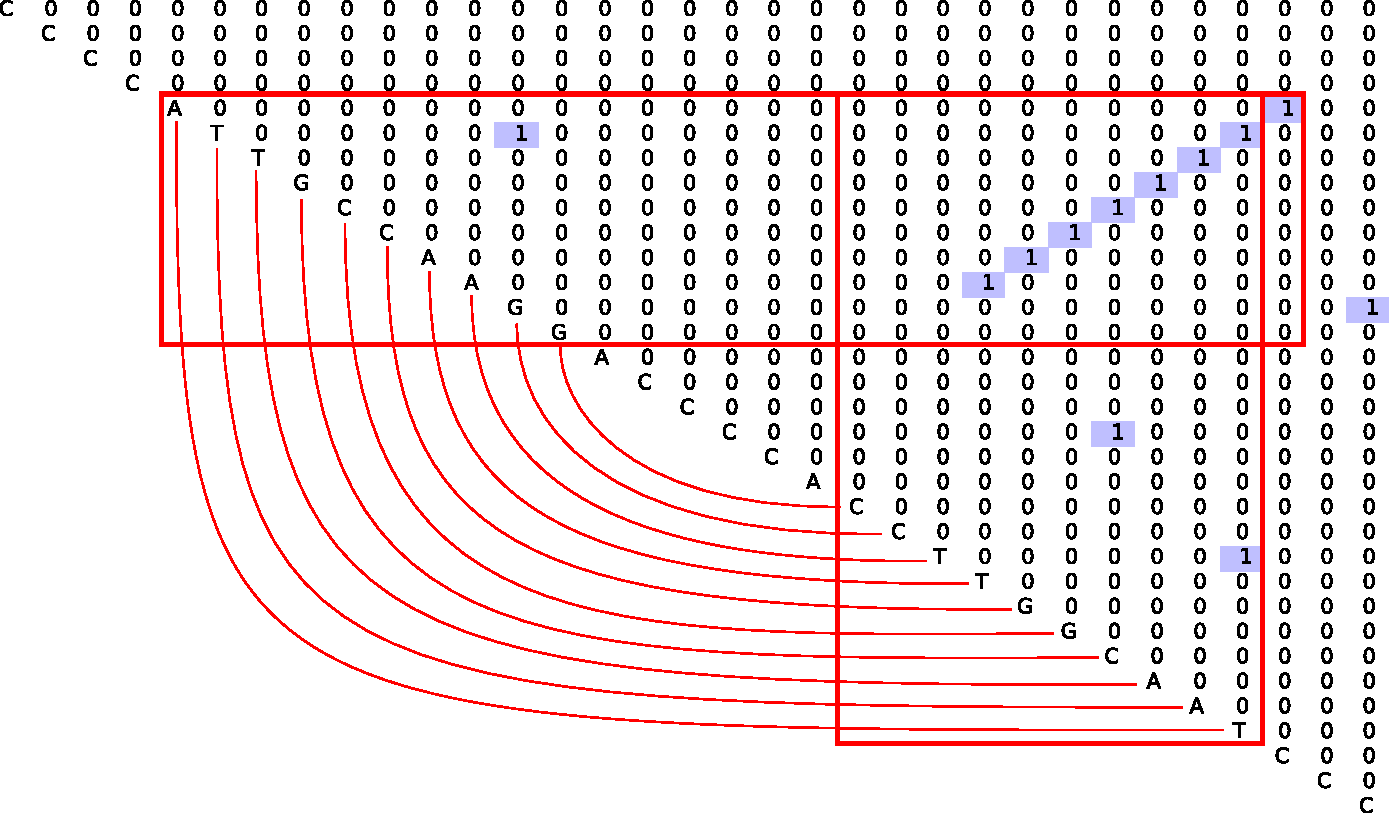
\includegraphics[width=.8\textwidth]{pictures/4.pdf}}
\onslide<2-3>{
\tikz[overlay,remember picture]{
\draw[draw=red,thick,fill opacity=0.2] ($(xx) + (1.1,4.97)$) rectangle ($(xx) + (9.05,3.235)$);
}
}

\onslide<3>{
\tikz[overlay,remember picture]{
\draw[draw=red,thick,fill opacity=0.2] ($(xx) + (5.8,4.97)$) rectangle ($(xx) + (8.75,0.4)$);
}
}

\end{frame}

\begin{frame}[fragile] \frametitle{Example 2: Pseudoknot}
\centering
 \texttt{CC{\color{red}ACTTA}CC{\color{blue}TATGA}CC{\color{red}TAAGT}CC{\color{blue}TCATA}CC}
\vspace{1cm}

\tikzmark{y}{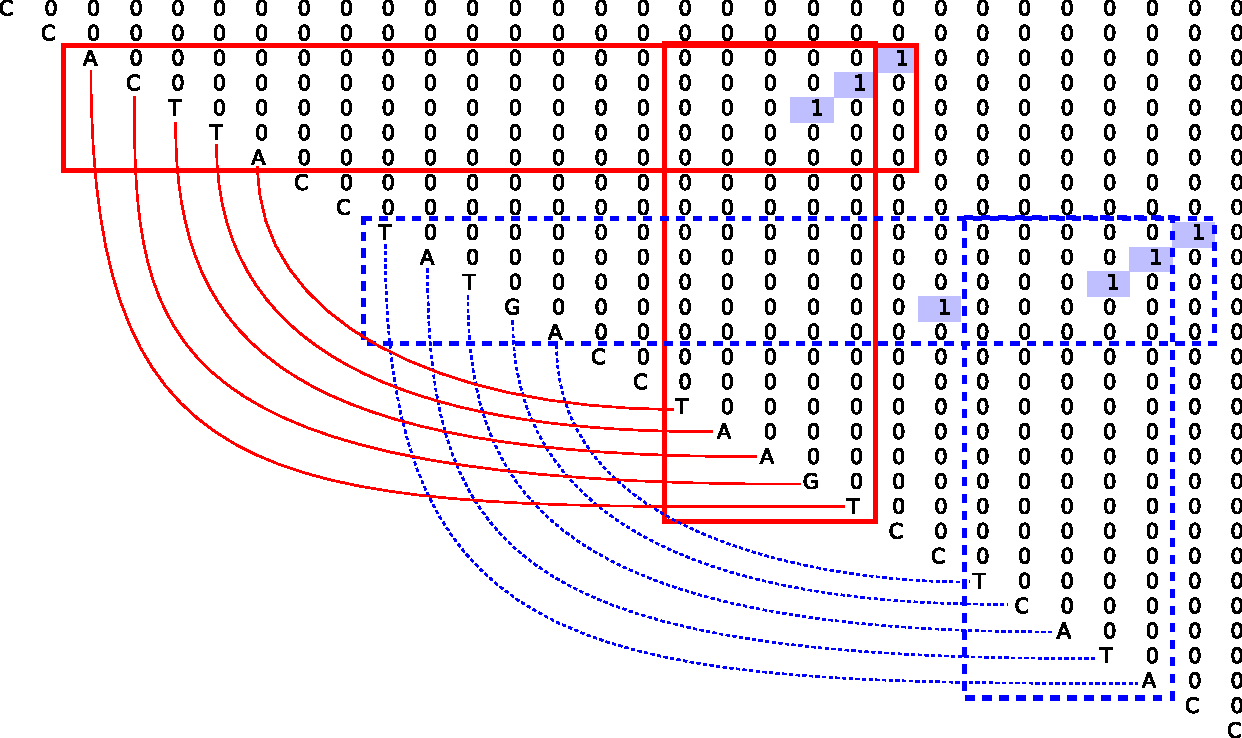
\includegraphics[width=.8\textwidth]{pictures/5.pdf}}

\onslide<2-3>{
\tikz[overlay,remember picture]{
\draw[draw=red,thick,fill opacity=0.2] ($(y) + (0.6,5.37)$) rectangle ($(y) + (7.15,4.4)$);
\draw[draw=red,thick,fill opacity=0.2] ($(y) + (5.15,5.37)$) rectangle ($(y) + (6.8,1.7)$);
}
}

\onslide<3>{
\tikz[overlay,remember picture]{
\draw[draw=blue,thick,fill opacity=0.2] ($(y) + (2.8,4.01)$) rectangle ($(y) + (9.42,3.05)$);
\draw[draw=blue,thick,fill opacity=0.2] ($(y) + (7.45,4.01)$) rectangle ($(y) + (9.1,0.3)$);
}
}

\end{frame}


\begin{frame}[fragile] \frametitle{Example 3: real tRNA}
\centering
 \texttt{CAGGGCATAACCTAGCCCAACCTTGCCAAGG\\TTGGGGTCGAGGGTTCGAATCCCTTCGCCCGCTCCA}
\vspace{0.5cm}
\begin{itemize}
  \item Novosphingobium aromaticivorans DSM 12444 chr.trna57-GlyGCC(268150-268084) Gly (GCC) 67 bp Sc: 22.9, from \href{http://gtrnadb2009.ucsc.edu/download.html}{GtRNAdb}
  \item Predicted secondary structures are given by using the \href{http://rna.urmc.rochester.edu/RNAstructureWeb/Servers/Fold/Fold.html}{Fold Web Server with default settings}

\end{itemize}
\end{frame}

\begin{frame}[fragile] \frametitle{Example 3: real tRNA}
\centering

\tikzmark{an}{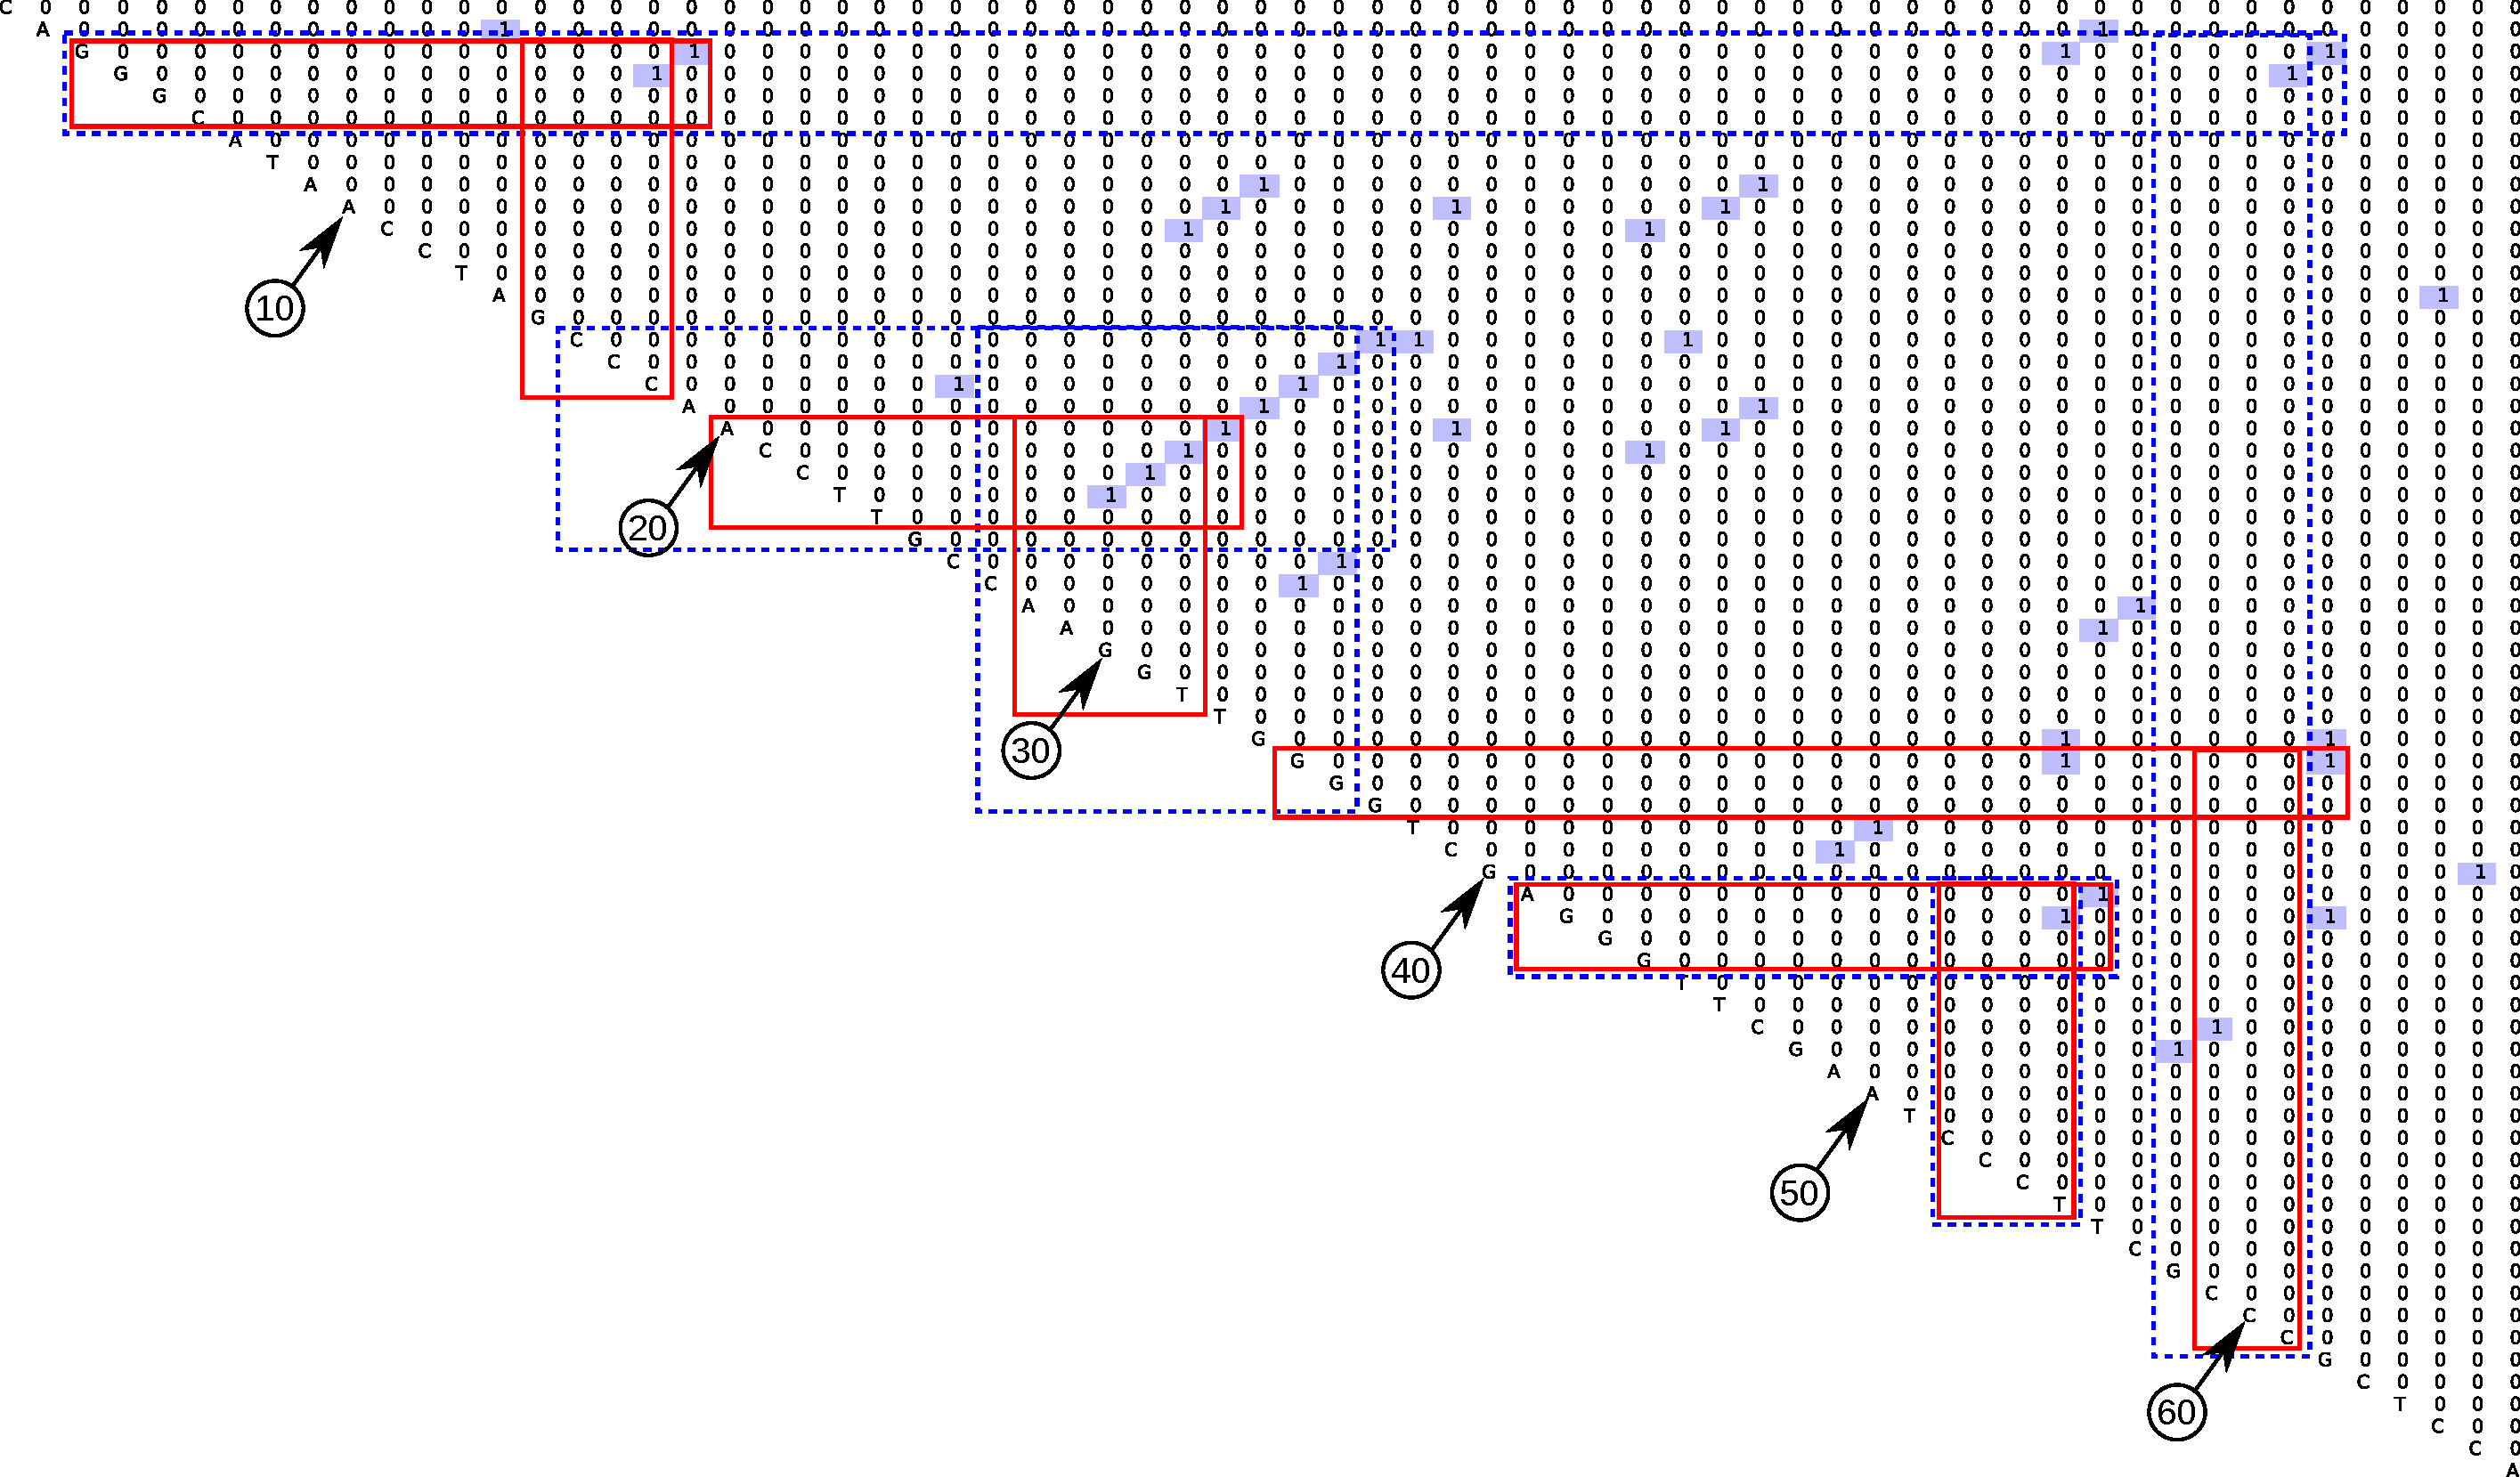
\includegraphics[width=\textwidth]{pictures/0m.pdf}}

\onslide<2-3>{\Put(-175,150){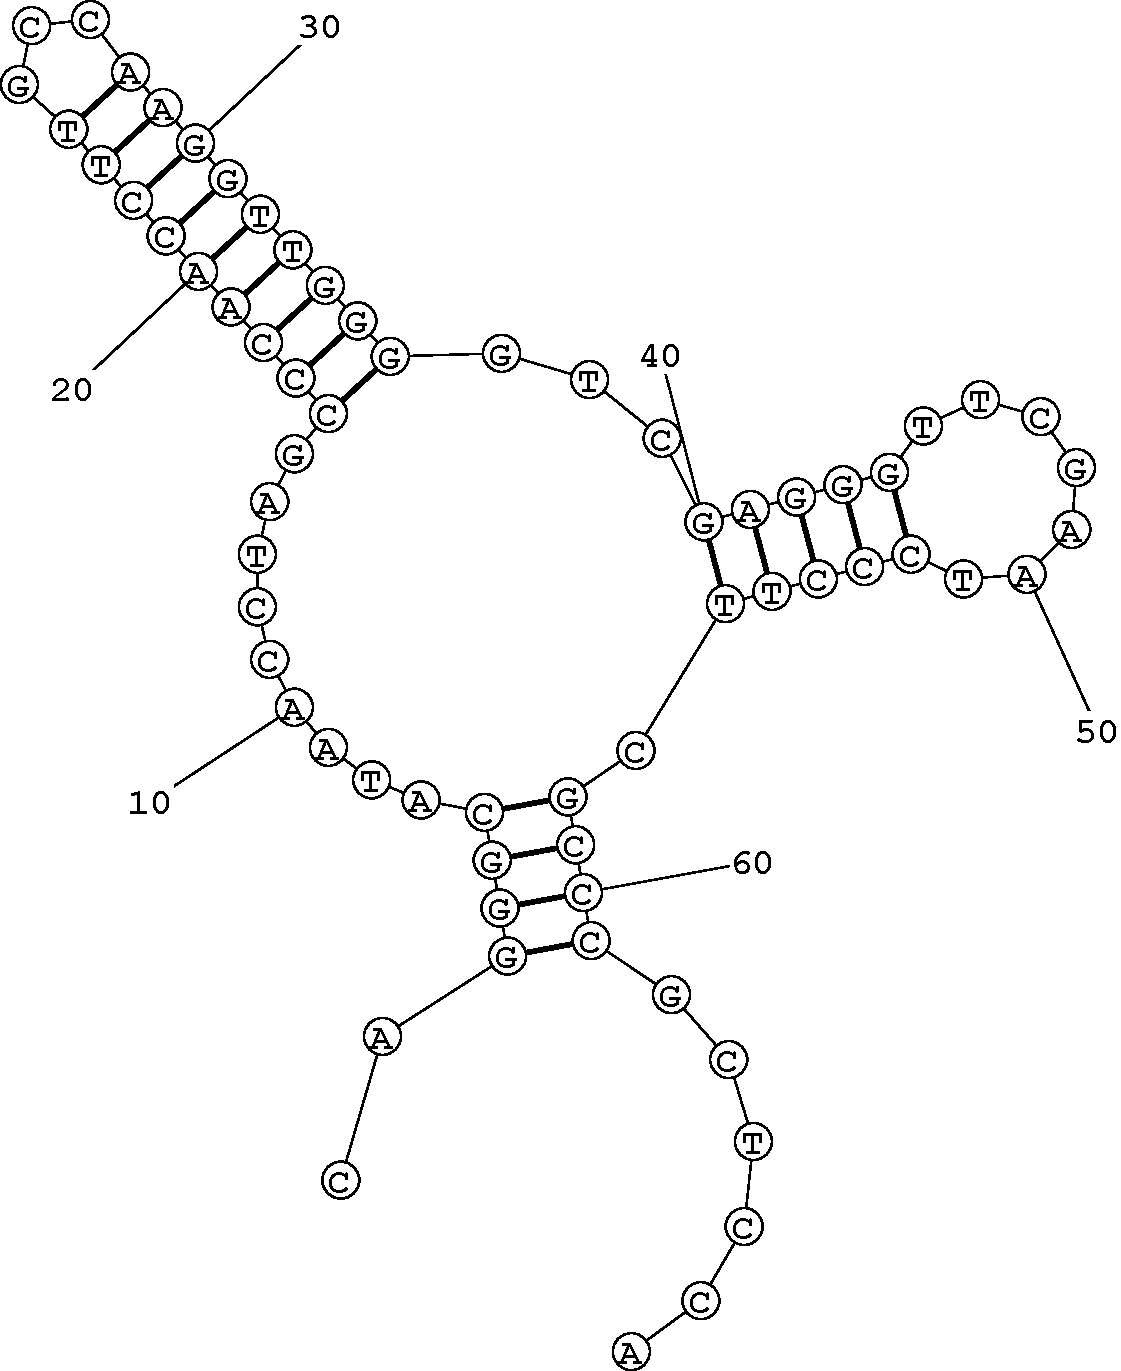
\includegraphics[height=6cm]{pictures/Fold1.pdf}}}
\onslide<3-3,7>{
\tikz[overlay,remember picture]{
\draw[draw=blue,thick,fill opacity=0.2] ($(an) + (0.28,6.885)$) rectangle ($(an) + (11.22,6.415)$);
\draw[draw=blue,thick,fill opacity=0.2] ($(an) + (10.3,6.885)$) rectangle ($(an) + (11.025,0.57)$);

\draw[draw=blue,thick,fill opacity=0.2] ($(an) + (2.65,5.49)$) rectangle ($(an) + (6.68,4.42)$);
\draw[draw=blue,thick,fill opacity=0.2] ($(an) + (4.65,5.49)$) rectangle ($(an) + (6.46,3.2)$);

\draw[draw=blue,thick,fill opacity=0.2] ($(an) + (7.2,2.85)$) rectangle ($(an) + (10.12,2.4)$);
\draw[draw=blue,thick,fill opacity=0.2] ($(an) + (9.23,2.85)$) rectangle ($(an) + (9.95,1.2)$);
}
}

\onslide<5-6>{\Put(-10,130){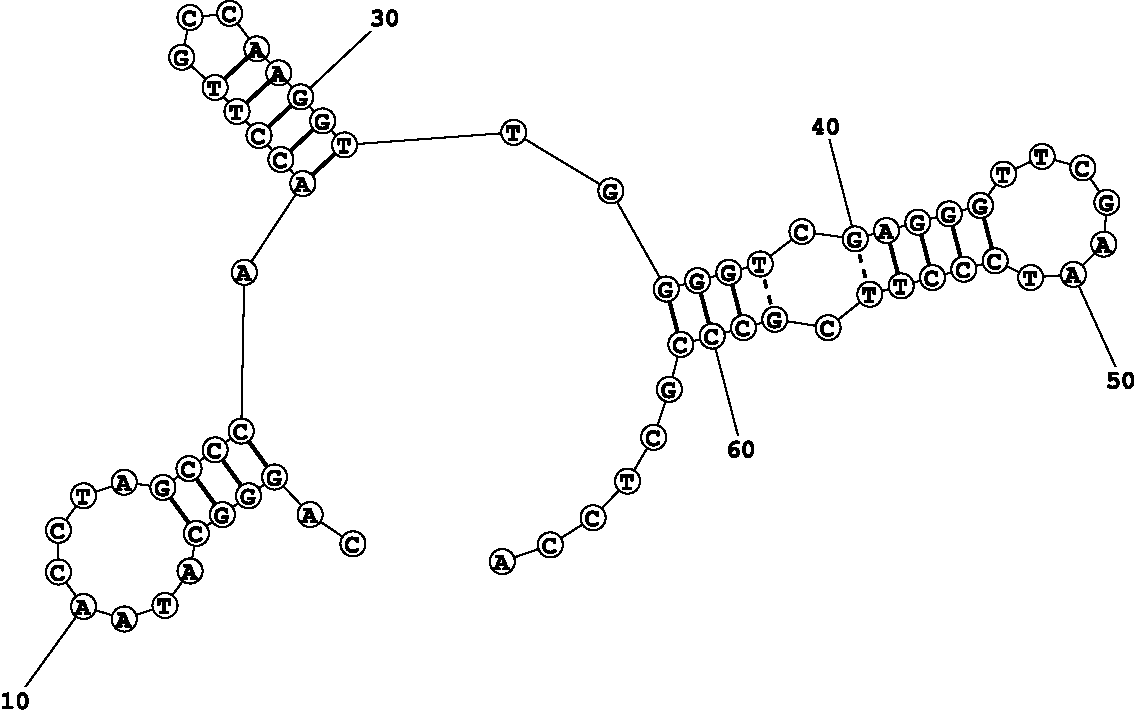
\includegraphics[height=4.3cm]{pictures/Fold2.pdf}}}
\onslide<6-7>{
\tikz[overlay,remember picture]{

\draw[draw=red,thick,fill opacity=0.2] ($(an) + (0.31,6.86)$) rectangle ($(an) + (3.4,6.44)$);
\draw[draw=red,thick,fill opacity=0.2] ($(an) + (2.5,6.86)$) rectangle ($(an) + (3.2,5.1)$);

\draw[draw=red,thick,fill opacity=0.2] ($(an) + (3.4,5.06)$) rectangle ($(an) + (5.95,4.535)$);
\draw[draw=red,thick,fill opacity=0.2] ($(an) + (4.83,5.06)$) rectangle ($(an) + (5.73,3.6)$);

\draw[draw=red,thick,fill opacity=0.2] ($(an) + (6.1,3.47)$) rectangle ($(an) + (11.2,3.15)$);
\draw[draw=red,thick,fill opacity=0.2] ($(an) + (10.5,3.47)$) rectangle ($(an) + (11,0.6)$);

\draw[draw=red,thick,fill opacity=0.2] ($(an) + (7.2,2.85)$) rectangle ($(an) + (10.12,2.4)$);
\draw[draw=red,thick,fill opacity=0.2] ($(an) + (9.23,2.85)$) rectangle ($(an) + (9.95,1.2)$);
}
}
\end{frame}

\begin{frame} \frametitle{Summary}

\begin{itemize}
  \item Parser is only a features extractor
  \item Parsing result contains all possible foldings (w.r.t. grammar) including impossible in practice
  \item Grammar is a parameter: one can add a \texttt{G-T} pair, change minimal height of the stem, etc
  \item It is possible to detect features which are not expressible in the language class in use
\end{itemize}

\end{frame}

\begin{frame} \frametitle{Artificial Neural Networks}

\begin{itemize}
  \item Dense neural network
  \begin{itemize}
    \item About 10 dense layers
    \item \texttt{Relu} activation function
  \end{itemize}
  \item Problem: input size is fixed, but the length of sequences is variable \\
  \begin{center}
  \begin{minipage}[t]{0.28\textwidth}
    \texttt{ACACAC \\
    CGTACGCT \\
    GCT}
  \end{minipage}~
  \begin{minipage}[m]{0.18\textwidth}
    \vspace{1cm}
    $\Rightarrow$
  \end{minipage}~
  \begin{minipage}[t]{0.28\textwidth}
    \texttt{ACACAC\$\$ \\
    CGTACGCT \\
    GCT\$\$\$\$\$}
  \end{minipage}
\end{center}

  \item Agressive dropout (up to 90\% after each layer) and batch normalization (after each layer) for learning stabilization
\end{itemize}

\end{frame}

\begin{frame} \frametitle{Evaluation: 16s rRNA detection}
\begin{itemize}
 \item Training data
 \begin{itemize}
   \item All sequences are 512 symbols in length
   \item Totally up to 310000 sequences
  \item Positive: random subsequences of 16s rRNA sequences from the Green Genes database
  \item Negative: random subsequences of full genes from the NCBI database
 \end{itemize}
\item Validation set: up to 81000 sequences
\item Accuracy is 90\% after training
\end{itemize}

\end{frame}

\begin{frame} \frametitle{Evaluation: tRNA classification}
\begin{itemize}
 \item Training data: 50000 sequences from GtRNADB
 \item Input data normalization
 \begin {itemize}
    \item Set the upper bound of sequence length to 220
    \item First $k$ symbols of the input are tRNA and the rest $220 - k$ symbols are filled by the special symbol
\end{itemize}

\item Validation set:  217984 sequences for prokaryotes and 62656 sequences for eukaryotes from tRNADB-CE 3
\item Accuracy is 97\% after training
\begin{itemize}
  \item 3276 of eukaryotes (5.23\% of all eukaryotes in the validation set) are classified as prokaryotes \item 4373 of prokaryotes (2.01\% of all prokaryotes in the validation set) are classified as eukaryotes
\end{itemize}

\end{itemize}

\end{frame}


\begin{frame} \frametitle{Future work}

\begin{itemize}
 \item Create DNN which does not requre input parsing
 \begin{itemize}
   \item Create a training set of matrices using parsing
   \item Train the network $NN_1$ which can handle vectorized matrices
   \item Create network $NN_2$ by extending $NN_1$ with a set of layers which convert the sequence to input for $NN_1$
   \item Train $NN_2$, weights of layers from $NN_1$ are fixed
 \end{itemize}
 \item Try to use other types of neural networks: bitwise networks, convolutional networks
 \item Do more evaluation
 \item Perform comparison with other tools
\end{itemize}

\end{frame}

\begin{frame} \frametitle{Conclusion}

\begin{itemize}
 \item We propose the approach to handle secondary structure of sequences
 \item This approach can be applied for real data processing
 \item This approach can be extended to more expressive classes of formal languages
 \begin{itemize}
   \item Conjunctive and boolean grammars
   \item Multiple context-free grammars
 \end{itemize}
\end{itemize}

\end{frame}


\begin{frame}
%\transwipe[direction=90]
\frametitle{Contact Information}
\begin{itemize}
  \item Semyon Grigorev:
    \begin{itemize}
      \item \href{mailto:s.v.grigoriev@spbu.ru}{s.v.grigoriev@spbu.ru}
      \item \href{mailto:Semen.Grigorev@jetbrains.com}{Semen.Grigorev@jetbrains.com}
    \end{itemize}
  \item Polina Lunina:
  \begin{itemize}
    \item  \href{mailto:lunina_polina@mail.ru}{lunina\_polina@mail.ru}
  \end{itemize}
  \item Trained models: \href{https://github.com/YaccConstructor/YC.Bio}{https://github.com/YaccConstructor/YC.Bio}
\end{itemize}
\vspace{2cm}
\center{\huge{Thanks!}}
\end{frame}
\end{document}
